\begin{name}
	{Biên soạn \& Phản biện: Thầy Trương Quan Kía, Thầy Thành Đức Trung, Thầy Nguyễn Văn Nay}
	{Đề thi thử THPT Quốc Gia Lần 1 môn Toán THPT - Phan Đình Phùng - Hà Nội, năm 2020 - 2021}
\end{name}
	\setcounter{ex}{0}
	\Opensolutionfile{ans}[ans/ans-2-GHK1-25-PhanDinhPhung-HaNoi-21-L1]	
\begin{ex}%[Thi thử L1, THPT Phan Đình Phùng, 2020]%[Trương Quan Kía, dự án 12EX3]%[2D1Y1-2]
	Cho hàm số $y=f(x)$ có bảng biến thiên như sau.
	\begin{center}
		
\begin{tikzpicture}[>=stealth]
		\tkzTabInit[nocadre=false,lgt=1.2,espcl=2.5,deltacl=0.5]{$x$/.7 ,$f'(x)$/.7,$f(x)$/1.8}
		{$-\infty$ , $-1$ , $1$ , $+\infty$}
		\tkzTabLine{ , + , $0$ , - , $0$ , + , }
		\tkzTabVar{-/$-\infty$ , +/$4$ , -/$0$ , +/$+\infty$}
		\end{tikzpicture}
	\end{center}
	Hàm số đã cho nghịch biến trên khoảng nào dưới đây?
	\choice
	{$(0 ; 2)$}
	{$(-\infty ;-1)$}
	{\True $(-1 ; 1)$}
	{$(0 ; 4)$}
	\loigiai{
		Hàm số đã cho nghịch biến trên khoảng $(-1;1)$.
	}
\end{ex}
\begin{ex}%[Thi thử L1, THPT Phan Đình Phùng - Hà Nội, 2021]%[Thành Đức Trung, 12EX3]%[2D1Y2-2]
	Cho hàm số $y = f(x)$ có bảng xét dấu $f'(x)$ như sau
	\begin{center}
		
\begin{tikzpicture}[scale = 0.8, font=\footnotesize, line join=round, line cap=round, >=stealth]
		\tkzTabInit[nocadre=false,lgt=1.6, espcl=2.2, deltacl=0.6]{$x$ /0.9, $f'(x)$ /0.9}{$-\infty$, $-2$, $0$, $1$, $2$, $+\infty$}
		\tkzTabLine{,-,0,-,0,+,0,-,0,+,}
		\end{tikzpicture}
	\end{center}
	Số điểm cực tiểu của hàm số $y = f (x)$ là
	\choice
	{$4$}
	{$1$}
	{$3$}
	{\True $2$}
	\loigiai{
		Dựa vào bảng biến thiên, ta thấy đạo hàm đổi dấu từ âm sang dương 2 lần nên hàm số đã cho có 2 điểm cực tiểu.
	}
\end{ex}
\begin{ex}%[Thi thử L1, THPT Phan Đình Phùng, 2020]%[Trương Quan Kía, dự án 12EX3]%[2D1Y3-1]
	\immini
	{
		Cho hàm số $y=f(x)$ có đồ thị như hình vẽ
		Mệnh đề nào dưới đây \textbf{sai}?
		\choice
		{$\max\limits_{[-2 ; 2]}f(x)=f(2)$}
		{$\min\limits_{[-2 ; 2]}f(x)=f(1)$}
		{$\max\limits_{[-2 ; 2]}f(x)=f(-2)$}
		{\True $\min\limits_{[-2 ; 2]}f(x)=f(0)$}
	}
	{
		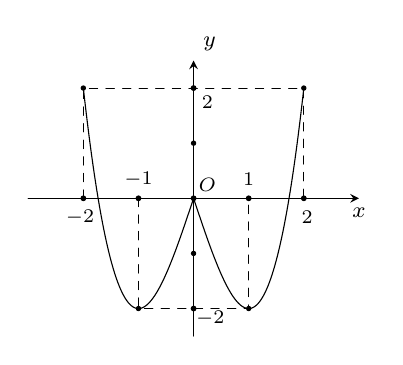
\begin{tikzpicture}[scale=0.7, font=\footnotesize, line join=round, line cap=round, >=stealth]
		\draw[->] (-3,0)--(3,0)node[below]{$x$};
		\draw[->] (0,-2.5)--(0,2.5)node[above right]{$y$};
		\draw[dashed](-2,0)|-(0,2)-|(2,0)(-1,0)|-(0,-2)-|(1,0);
		\draw[samples=300,domain=0:2,smooth] plot (\x, {(\x)^3-3*(\x)});
		\draw[samples=300,domain=-2:0,smooth] plot (\x, {-(\x)^3+3*(\x)});
		\foreach \x/\y/\g/\z in{-2/0/-100/-2,-1/0/90/-1,0/0/45/O,1/0/90/1,2/0/-80/2,0/-2/-30/-2,0/2/-45/2}
		\draw[fill=black](\x,\y)node[shift={(\g:7pt)}]{\scriptsize$\z$}circle(1.2pt);
		\foreach \x/\y in{-2/2,0/1,2/2,0/-1,-1/-2,1/-2}
		\draw[fill=black](\x,\y)circle(1.1pt);
		\end{tikzpicture}
	}
	\loigiai{
		Dựa vào đồ thị ta suy ra $\max\limits_{[-2 ; 2]}f(x)=f(2)=f(-2)$ và $\min\limits_{[-2 ; 2]}f(x)=f(-1)=f(1)$.\\
		Vậy mệnh đề \textbf{sai} là $\min\limits_{[-2 ; 2]}f(x)=f(0)$. 
	}
\end{ex}
\begin{ex}%[Thi thử L1, THPT Phan Đình Phùng, 2020]%[Trương Quan Kía, dự án 12EX3]%[2D1Y5-4]
	Số giao điểm của hai đồ thị hàm số $y=f(x)$ và $y=g(x)$ bằng số nghiệm phân biệt của phương trình nào sau đây?
	\choice
	{$\dfrac{f(x)}{g(x)}=0$}
	{$f(x)+g(x)=0$}
	{\True $f(x)-g(x)=0$}
	{$f(x)\cdot g(x)=0$}
	\loigiai{
		Số giao điểm của hai đồ thị hàm số $y=f(x)$ và $y=g(x)$ bằng số nghiệm phân biệt của phương trình \[f(x)=g(x)\Leftrightarrow f(x)-g(x)=0.\]
	}
\end{ex}
\begin{ex}%[Thi thử L1, THPT Phan Đình Phùng - Hà Nội, 2021]%[Thành Đức Trung, 12EX3]%[2D1Y5-7]
	Với giá trị nào của $m$ thì đồ thị hàm số $y = \dfrac{2x^2 + 6mx + 4}{mx + 2}$ đi qua điểm $A(-1;4)$?
	\choice
	{$m = 2$}
	{$m = 1$}
	{\True $m = -1$}
	{$m = \dfrac{1}{2}$}
	\loigiai{
		Đồ thị hàm số $y = \dfrac{2x^2 + 6mx + 4}{mx + 2}$ đi qua điểm $A(-1;4)$ nên ta có
		\[4 = \dfrac{2\cdot\left(-1\right)^2 + 6m\cdot\left(-1\right) + 4}{m\cdot\left(-1\right) + 2}\Leftrightarrow 4 = \dfrac{6 - 6m}{2 - m}\Leftrightarrow m = -1.\]
	}
\end{ex}
\begin{ex}%[Thi thử L1, THPT Phan Đình Phùng, 2020]%[Trương Quan Kía, dự án 12EX3]%[2D2Y1-2]
	Cho $a$ là số thực dương và $m$, $n$ là các số thực tùy ý. Trong các tính chất sau, tính chất nào đúng?
	\choice
	{$a^m+a^n=a^{m+n}$}
	{$a^m\cdot a^n=a^{m\cdot n}$}
	{\True $a^m\cdot a^n=a^{m+n}$}
	{$a^m+a^n=a^{m\cdot n}$}
	\loigiai{
		Theo lý thuyết ta có $a^m\cdot a^n=a^{m+n}$.
	}
\end{ex}
\begin{ex}%[Thi thử L1, THPT Phan Đình Phùng, 2020]%[Trương Quan Kía, dự án 12EX3]%[2H1Y1-2]
	Số cạnh của một hình tứ diện là
	\choice
	{$9$}
	{$8$}
	{$4$}
	{\True $6$}
	\loigiai{
		\immini
		{
			Số cạnh của một hình tứ diện là $6$.
		}
		{
			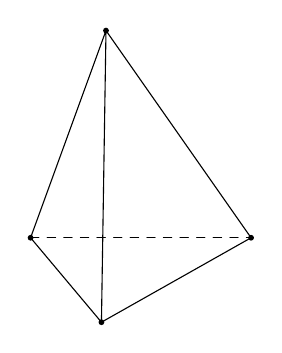
\begin{tikzpicture}[scale=0.7, font=\footnotesize, line join=round, line cap=round, >=stealth]
			\def\ac{4} % cạnh AC
			\def\ab{2} % cạnh AB
			\def\as{4} % cạnh AS
			\def\gocA{50} % góc A của đáy
			\coordinate (A) at (0,0);
			\coordinate (C) at (\ac,0);
			\coordinate (B) at (-\gocA:\ab);
			\coordinate (S) at (70:\as);
			\draw (A)--(B)--(C)--(S)--cycle (S)--(B);
			\draw[dashed] (A)--(C);
			\foreach \diem in {A,B,C,S}\fill (\diem)circle(1.5pt);
			\end{tikzpicture}
			
		}
	}
\end{ex}
\begin{ex}%[Thi thử L1, THPT Phan Đình Phùng, 2020]%[Trương Quan Kía, dự án 12EX3]%[2H1Y3-2]
	Thề tích khối lập phương có cạnh bằng $3a$ là
	\choice
	{\True $27a^3$}
	{$3a^3$}
	{$a^3$}
	{$9a^3$}
	\loigiai{
		Ta có $V=\text{cạnh}^3=\left(3a\right)^3=27a^3$.
	}
\end{ex}
\begin{ex}%[Thi thử L1, THPT Phan Đình Phùng, 2020]%[Trương Quan Kía, dự án 12EX3]%[2H1Y3-2]
	Công thức tính thể tích khối chóp có diện tích đáy $B$ và chiều cao $h$ là
	\choice
	{$V=\dfrac{1}{2}Bh$}
	{$V=\dfrac{1}{6}Bh$}
	{$V=Bh$}
	{\True $V=\dfrac{1}{3}Bh$}
	\loigiai{
		
	}
\end{ex}
\begin{ex}%[Thi thử L1, THPT Phan Đình Phùng, 2020]%[Trương Quan Kía, dự án 12EX3]%[2H2Y2-1]
	Công thức tính thể tích khối cầu bán kính $R$ là
	\choice
	{\True $V=\dfrac 43\pi R^3$}
	{$V=4\pi R^2$}
	{$V=4\pi R^3$}
	{$V=\dfrac 34\pi R^3$}
	\loigiai{
		Công thức tính thể tích khối cầu bán kính $R$ là $V=\dfrac 43\pi R^3$.
	}
\end{ex}
\begin{ex}%[Thi thử L1, THPT Phan Đình Phùng, 2020]%[Trương Quan Kía, dự án 12EX3]%[2H2Y2-1]
	Số điểm chung giữa mặt cầu và mặt phẳng không thể là
	\choice
	{$0$}
	{$1$}
	{\True $2$}
	{Vô số}
	\loigiai{
Mặt cầu và mặt phẳng có $3$	vị trí tương đối là
\begin{itemize}
	\item Mặt cầu không cắt mặt phẳng $\Rightarrow$ số điểm chung là $0$.
	\item Mặt cầu tiếp xúc mặt phẳng $\Rightarrow$ số điểm chung là $1$.
	\item Mặt cầu cắt mặt phẳng theo giao tuyến là đường tròn $\Rightarrow$ số điểm chung là vô số.
\end{itemize}	
	}
\end{ex}
\begin{ex}%[Thi thử L1, THPT Phan Đình Phùng - Hà Nội, 2021]%[Thành Đức Trung, 12EX3]%[1D5B2-2]
	Cho đường cong $\left(C\right)$ có phương trình $y = \dfrac{x - 1}{x + 1}$. Gọi $M$ là giao điểm của $\left(C\right)$ với trục tung. Tiếp tuyến của $\left(C\right)$ tại $M$ có phương trình
	\choice
	{$y = x - 2$}
	{$y = 2x + 1$}
	{$y = -2x - 1$}
	{\True $y = 2x - 1$}
	\loigiai{
		Ta có $y' = \dfrac{2}{(x + 1)^2}$ và $M\left(0;-1\right)$.\\
		Hệ số góc của tiếp tuyến là $k = f'\left(0\right) = 2$. Suy ra phương trình tiếp tuyến của $\left(C\right)$ tại $M$ là \[y = 2(x - 0) - 1 = 2x - 1.\]
	}
\end{ex}
\begin{ex}%[Thi thử L1, THPT Phan Đình Phùng, 2020]%[Trương Quan Kía, dự án 12EX3]%[2D1B1-1]
	Cho hàm số $f(x)=\dfrac{2 x+1}{x-3}$. Chọn mệnh đề \textbf{sai} trong các mệnh đề sau đây?
	\choice
	{Hàm số nghịch biến trên khoảng $(-\infty ; 3)$}
	{\True Hàm số nghịch biến trên $\mathbb{R} \setminus \{3\}$}
	{Hàm số nghịch biến trên các khoảng $(-\infty ; 3)$ và $(3 ;+\infty)$}
	{Hàm số nghịch biến trên khoảng $(3 ;+\infty)$}
	\loigiai{
		Ta có $y'=\dfrac{-7}{\left(x-3\right)^2}<0$, $\forall x\ne 3$.\\
		Vậy hàm số đã cho nghịch biến trên các khoảng $(-\infty ; 3)$ và $(3 ;+\infty)$.
	}
\end{ex}
\begin{ex}%[Thi thử L1, THPT Phan Đình Phùng - Hà Nội, 2021]%[Thành Đức Trung, 12EX3]%[2D1B1-1]
	Tìm tất cả các giá trị thực của tham số $m$ để hàm số $y = \dfrac{x - m}{x + 1}$ đồng biến trên từng khoảng xác định.
	\choice
	{$m\ge -1$}
	{$m > 1$}
	{$m\ge 1$}
	{\True $m > -1$}
	\loigiai{
		Ta có $y' = \dfrac{1 + m}{(x + 1)^2}$.\\
		Để hàm số đồng biến trên từng khoảng xác định thì $1 + m > 0\Leftrightarrow m > -1$.
	}
\end{ex}
\begin{ex}%[Thi thử L1, THPT Phan Đình Phùng - Hà Nội, 2021]%[Thành Đức Trung, 12EX3]%[2D1B2-3]
	Gọi $A$ là điểm cực đại của đồ thị hàm số $y = 2x^3 - 3x^2 - 1$ thì $A$ có tọa độ là
	\choice
	{$A\left(-1;-6\right)$}
	{\True $A\left(0;-1\right)$}
	{$A\left(1;-2\right)$}
	{$A\left(2;3\right)$}
	\loigiai{
		Ta có $y'(x) = 6x^2 - 6x = 0 \Leftrightarrow \hoac{&x = 0\\&x = 1.}$\\
		Lại có $\heva{&y''(0) = -6 < 0\\&y''(1) = 6 > 0}$ nên $x = 0$ là điểm cực đại của hàm số.\\ 
		Vậy đồ thị hàm số có điểm cực đại là $A(0;-1)$.
	}
\end{ex}
\begin{ex}%[Thi thử L1, THPT Phan Đình Phùng, 2020]%[Trương Quan Kía, dự án 12EX3]%[2D1B2-5]
	Tìm điều kiện của tham số $b$ để hàm số $y=x^4+b x^2+c$ có $3$ điểm cực trị?
	\choice
	{$b=0$}
	{$b\neq 0$}
	{\True $b<0$}
	{$b>0$}
	\loigiai{
		Hàm số $y=x^4+bx^2+c$ có $3$ điểm cực trị $\Leftrightarrow a\cdot b<0\Leftrightarrow b<0$.
	}
\end{ex}
\begin{ex}%[Thi thử L1, THPT Phan Đình Phùng - Hà Nội, 2021]%[Thành Đức Trung, 12EX3]%[2D1B2-5]
	Tìm tất cả các giá trị của tham số $m$ để hàm số $y = mx^4 + (m - 3)x^2 + 3m - 5$ chỉ có cực tiểu mà không có cực đại.
	\choice
	{$\hoac{&m \le 0\\&m > 3}$}
	{$m\le 0$}
	{$0\le m\le 3$}
	{\True $m > 3$}
	\loigiai{
		\begin{itemize}
			\item Với $m = 0$ thì hàm số trở thành $y = -3x^2 + 3m - 5$. Dễ thấy đồ thị là một parabol quay bề lõm xuống dưới, do đó hàm số chỉ có cực đại mà không có cực tiểu.
			\item Với $m\neq 0$ thì hàm số có một cực tiểu mà không có cực đại khi và chỉ khi
			\[\heva{&m > 0\\&m(m - 3) \ge 0}\Leftrightarrow m>3.\]
		\end{itemize}
		Vậy $m > 3$ là các giá trị thỏa mãn đề bài.
	}
\end{ex}
\begin{ex}%[Thi thử L1, THPT Phan Đình Phùng - Hà Nội, 2021]%[Thành Đức Trung, 12EX3]%[2D1B3-1]
	Biết rằng giá trị nhỏ nhất của hàm số $f(x) = \dfrac{mx + 5}{x - m}$ trên đoạn $\left[0;1\right]$ bằng $-7$. Mệnh đề nào sau đây đúng?
	\choice
	{$-1\le m \le 1$}
	{$0 < m < 1$}
	{\True $0 < m \le 2$}
	{$-1 < m < 0$}
	\loigiai{
		Điều kiện: $m\notin\left[0;1\right]$.\\
		Ta có $f'(x) = \dfrac{-m^2 - 5}{(x - m)^2} < 0$, $\forall x\neq m$. Do đó hàm số nghịch biến trên $\left[0;1\right]$.\\
		Suy ra $\displaystyle\min_{x\in\left[0;1\right]} f(x) = f(1)\Leftrightarrow \dfrac{m + 5}{1 - m} = -7\Leftrightarrow m = 2\in\left(0;2\right]$.
	}
\end{ex}
\begin{ex}%[Thi thử L1, THPT Phan Đình Phùng, 2020]%[Trương Quan Kía, dự án 12EX3]%[2D1B4-1]
	Tìm phương trình đường tiệm cận ngang của đồ thị hàm số $y=\dfrac{3x+2}{x+1}$.
	\choice
	{\True $y=3$}
	{$x=-1$}
	{$x=3$}
	{$y=2$}
	\loigiai{
		Đường tiệm cận ngang của đồ thị hàm số $y=\dfrac{3x+2}{x+1}$ là $y=\dfrac{a}{c}=3$.
	}
\end{ex}
\begin{ex}%[Thi thử L1, THPT Phan Đình Phùng - Hà Nội, 2021]%[Thành Đức Trung, 12EX3]%[2D1B4-1]
	Số đường tiệm cận của đồ thị hàm số $y = \dfrac{x}{x^2 - 1}$ là
	\choice
	{$1$}
	{\True $3$}
	{$2$}
	{$4$}
	\loigiai{
		\begin{itemize}
			\item $\displaystyle\lim_{x\to\pm\infty}\dfrac{x}{x^2 - 1} = 0$. Suy ra $y = 0$ là tiệm cận ngang của đồ thị hàm số.
			\item $\displaystyle\lim_{x\to1^+}\dfrac{x}{x^2 - 1} = +\infty$; $\displaystyle\lim_{x\to1^-}\dfrac{x}{x^2 - 1} = -\infty$. Suy ra $x = 1$ là tiệm cận đứng của đồ thị hàm số.
			\item $\displaystyle\lim_{x\to(-1)^+}\dfrac{x}{x^2 - 1} = +\infty$; $\displaystyle\lim_{x\to(-1)^-}\dfrac{x}{x^2 - 1} = -\infty$. Suy ra $x = -1$ là tiệm cận đứng của đồ thị hàm số.
		\end{itemize}	
		Vậy đồ thị hàm số có tất cả $3$ đường tiệm cận.
	}
\end{ex}
\begin{ex}%[Thi thử L1, THPT Phan Đình Phùng, 2020]%[Trương Quan Kía, dự án 12EX3]%[2D1B5-1]
	Đồ thị của hàm số nào sau đây luôn nằm dưới trục hoành?
	\choice
	{$y=-x^4-4x^2+1$}
	{\True $y=-x^4+2x^2-2$}
	{$y=-x^3-2x^2+x-1$}
	{$y=x^4+3x^2-1$}
	\loigiai{
		\immini
		{
			Đồ thị hàm số $y=-x^4+2x^2-2$ (tham khảo hình vẽ bên) là hàm trùng phương có hệ số $a=-1<0$ và có $y=-\left(x^2-1\right)^2-1<0$ nên sẽ luôn nằm phía dưới trục hoành.
		}
		{
			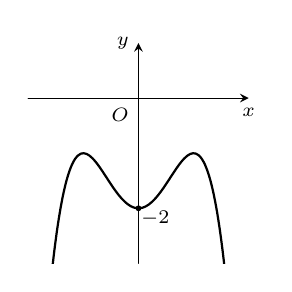
\begin{tikzpicture}[scale=0.7, font=\footnotesize, line join=round, line cap=round, >=stealth]
			\def\a{-1} % Hệ số a phải khác 0
			\def\b{2}
			\def\c{-2}
			%\draw[color=gray,dash pattern=on 1pt off 1pt,xstep=1.0cm,ystep=1.0cm] (-2,-3) grid (2,1);
			\draw[->] (-2,0) -- (2,0) node[below] {\scriptsize $x$};
			\draw[->] (0,-3) -- (0,1) node[left] {\scriptsize $y$};
			\draw (0,0)node[below left]{\scriptsize $O$};
			\clip (-2,-3)rectangle(2,1);
			\draw[thick,samples=150,smooth,domain=-4:4] plot(\x,{\a*(\x)^4+(\b)*(\x)^2+(\c)});
			\fill[black](0,-2)node[shift={(-30:7pt)}]{\scriptsize$-2$}circle(1.5pt);
			\end{tikzpicture}
		}
	}
\end{ex}
\begin{ex}%[Thi thử L1, THPT Phan Đình Phùng, 2020]%[Trương Quan Kía, dự án 12EX3]%[2D1B5-1]
	Bảng biến thiên ở hình bên là của hàm số nào trong bốn hàm số được liệt kê dưới đây?
	\begin{center}
		
\begin{tikzpicture}[>=stealth]
		\tkzTabInit[nocadre=false,lgt=1,espcl=3.5,deltacl=0.5]{$x$/.7 ,$y'$/.7,$y$/1.8}
		{$-\infty$ , $-1$ , $+\infty$}
		\tkzTabLine{ , + , d , + , }
		\tkzTabVar{-/$2$ , +D-/$+\infty$/$-\infty$ , +/$2$}
		\end{tikzpicture}
	\end{center}
	\choice
	{$y=\dfrac{-2x-3}{x-1}$}
	{$y=\dfrac{-x+1}{x-2}$}
	{\True $y=\dfrac{2x-3}{x+1}$}
	{$y=\dfrac{2x+3}{x+1}$}
	\loigiai{
		Từ bảng biến thiên ta suy ra đồ thị hàm số $y'>0$ và  tiệm cận ngang $y=2\Rightarrow$ chọn $y=\dfrac{2x-3}{x+1}$.
	}
\end{ex}
\begin{ex}%[Thi thử L1, THPT Phan Đình Phùng, 2020]%[Trương Quan Kía, dự án 12EX3]%[2D1B5-1]
	\immini
	{
		Đường cong trong hình bên là đồ thị của hàm số nào?
		\choice
		{$y=-x^3+3x^2+1$}
		{$y=x^3+3x^2+1$}
		{$y=-x^3-3x^2+1$}
		{\True $y=x^3-3x^2+1$}	
	}
	{
		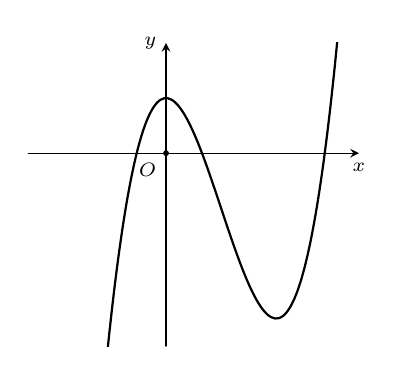
\begin{tikzpicture}[scale=0.7, font=\footnotesize, line join=round, line cap=round, >=stealth] 
		\def\a{1}\def\b{-3}\def\c{0}\def\d{1}
		\draw[->] (-2.5,0) -- (3.5,0)node[below]{\scriptsize $x$};
		\draw[->] (0,-3.5) -- (0,2) node[left] {\scriptsize $y$};
		\draw[fill=black] (0,0)node[below left]{\scriptsize $O$}circle(1.2pt);
		\clip (-2.5,-3.5)rectangle(3.5,2);
		\draw[thick,samples=150,smooth,domain=-5:5]plot(\x,{\a*(\x)^3+(\b)*(\x)^2+(\c)*\x+(\d)});
		\end{tikzpicture}
	}
	\loigiai{
		Từ hình vẽ ta suy ra đồ thị đã cho là hàm số bậc ba có $a>0$ và $2$ điểm cực trị $\Rightarrow$ chọn $y=x^3-3x^2+1$.
	}
\end{ex}
\begin{ex}%[Thi thử L1, THPT Phan Đình Phùng - Hà Nội, 2021]%[Thành Đức Trung, 12EX3]%[2D1B5-4]
	Đồ thị của hai hàm số $y = 4x^4 - 2x^2 + 1$ và $y = x^2 + x + 1$ có tất cả bao nhiêu điểm chung?
	\choice
	{\True $3$}
	{$1$}
	{$4$}
	{$2$}
	\loigiai{
		Xét phương trình hoành độ giao điểm của đồ thị hai hàm số
		\[
		\begin{aligned}
		4x^4 - 2x^2 + 1 = x^2 + x + 1 &\Leftrightarrow 4x^4 - 3x^2 - x = 0\\
		&\Leftrightarrow x\left(4x^3 - 3x - 1\right) = 0\\
		&\Leftrightarrow \hoac{&x = 0\\&x = 1\\&x = -\dfrac{1}{2}.}
		\end{aligned}
		\]
		Vậy đồ thị của hai hàm số $y = 4x^4 - 2x^2 + 1$ và $y = x^2 + x + 1$ có tất cả $3$ điểm chung.
	}
\end{ex}
\begin{ex}%[Thi thử L1, THPT Phan Đình Phùng - Hà Nội, 2021]%[Thành Đức Trung, 12EX3]%[2D2B1-1]
	Xét khẳng định: \lq\lq  Với mọi số thực $a$ và hai số hữu tỉ $r$, $s$, ta có $\left(a^r\right)^s = a^{rs}$\rq\rq. Với điều kiện nào trong các điều kiện sau thì khẳng định trên đúng?
	\choice
	{$a < 1$}
	{$a$ bất kì}
	{\True $a > 0$}
	{$a \neq 0$}
	\loigiai{
		Điều kiện để các biểu thức trên xác định là $a > 0$.
	}
\end{ex}
\begin{ex}%[Thi thử L1, THPT Phan Đình Phùng, 2020]%[Trương Quan Kía, dự án 12EX3]%[2D2B1-2]
	Cho số thực dương $a$. Sau khi rút gọn, biểu thức $P=\sqrt[3]{a \sqrt{a}}$ có dạng
	\choice
	{$\sqrt{a^3}$}
	{$\sqrt[3]{a}$}
	{\True $\sqrt{a}$}
	{$a$}
	\loigiai{
		Ta có $P=\sqrt[3]{a \sqrt{a}}=\left(
		a\cdot a^{\frac{1}{2}}\right)^{\frac{1}{3}}=\left(a^{\frac{3}{2}}\right)^{\frac{1}{3}}=a^{\frac{1}{2}}=\sqrt{a}$.
	}
\end{ex}
\begin{ex}%[Thi thử L1, THPT Phan Đình Phùng, 2020]%[Trương Quan Kía, dự án 12EX3]%[2D2B3-2]
	Cho số thực $a>0$ và $a \neq 1$. Tìm mệnh đề đúng trong các mệnh đề sau.
	\choice
	{$\log _{a}(x \cdot y)=\log _{a} x \cdot \log _{a} y$, ($\forall x, y>0$)}
	{\True $\log_a x^n=n\log_a x$, ($x>0, n\neq 0$)}
	{$\log_a 1=a$ và $\log_a a=0$}
	{$\log_a x$ có nghĩa với $\forall x \in \mathbb{R}$}
	\loigiai{
		Ta có $\log_a 1=a$ và $\log_a a=0$, với $a>0$, $a\ne 0$.\\
		Theo lý thuyết $\log_a x^n=n\log_a x$, ($x>0, n\neq 0$).
	}
\end{ex}
\begin{ex}%[Thi thử L1, THPT Phan Đình Phùng, 2020]%[Trương Quan Kía, dự án 12EX3]%[2D2B3-3]
	Nếu $a^{\frac{13}{7}}<a^{\frac{15}{8}}$ và $\log _{b} \left(\sqrt{2}+\sqrt{5}\right)>\log_{b} \left(2+\sqrt{3}\right)$ thì
	\choice
	{$0<a<1$ và $0<b<1$}
	{$0<a<1$ và $b>1$}
	{\True $a>1$ và $0<b<1$}
	{$a>1$ và $b>1$}
	\loigiai{
		Ta có $\heva{& a^{\frac{13}{7}}<a^{\frac{15}{8}} \\ & \dfrac{13}{7}<\dfrac{15}{8}}\Rightarrow a>1$.\\
		Mặt khác $\heva{& \log _{b} \left(\sqrt{2}+\sqrt{5}\right)>\log_{b} \left(2+\sqrt{3}\right) \\ & \sqrt{2}+\sqrt{5}<2+\sqrt{3}}\Rightarrow 0<b<1$.
	}
\end{ex}
\begin{ex}%[Thi thử L1, THPT Phan Đình Phùng - Hà Nội, 2021]%[Thành Đức Trung, 12EX3]%[2D2B3-3]
	Giả sử các biểu thức chứa logarit đều có nghĩa, hỏi mệnh đề nào sau đây đúng?
	\choice
	{$\log_a b > \log_a c \Leftrightarrow b > c$}
	{\True $\log_a b = \log_a c \Leftrightarrow b = c$}
	{$\log_a b < \log_a c \Leftrightarrow b < c$}
	{$\log_a b < \log_a c \Leftrightarrow b > c$}
	\loigiai{
		Mệnh đề đúng là \lq\lq  $\log_a b = \log_a c \Leftrightarrow b = c$\rq\rq.
	}
\end{ex}
\begin{ex}%[Thi thử L1, THPT Phan Đình Phùng - Hà Nội, 2021]%[Thành Đức Trung, 12EX3]%[2D2B3-4]
	Cho $0 < a \neq 1$, $b > 0$, $c > 0$ và $\log_a b = -2$, $\log_a c = 5$. Giá trị của $\log_a \dfrac{a\sqrt{b}}{\sqrt[3]{c}}$ là
	\choice
	{$-\dfrac{4}{3}$}
	{$-\dfrac{5}{3}$}
	{$-\dfrac{5}{4}$}
	{\True $-\dfrac{3}{5}$}
	\loigiai{
		Ta có $\log_a \dfrac{a\sqrt{b}}{\sqrt[3]{c}} = \log_a \left(a\sqrt{b}\right) - \log_a\sqrt[3]{c} = 1 + \dfrac{1}{2}\log_a b - \dfrac{1}{3}\log_a c = 1 + \dfrac{\left(-2\right)}{2} - \dfrac{3}{5} = -\dfrac{3}{5}$.
	}
\end{ex}
\begin{ex}%[Thi thử L1, THPT Phan Đình Phùng - Hà Nội, 2021]%[Thành Đức Trung, 12EX3]%[2H1B2-2]
	Trung điểm các cạnh của hình tứ diện đều tạo thành
	\choice
	{Lăng trụ tam giác đều}
	{\True Bát diện đều}
	{Hình lục giác đều}
	{Hình lập phương}
	\loigiai{
		\immini{
			Trung điểm các cạnh của hình tứ diện đều tạo thành hình bát diện đều.
		}{
			\begin{tikzpicture}[scale=1.4, line join = round, line cap = round]
			\tikzset{label style/.style={font=\footnotesize}}
			\tkzDefPoints{0/0/B,4/0/C,1/-1.5/D,1.5/2/A}
			\coordinate (M) at ($(A)!0.5!(B)$);
			\coordinate (N) at ($(A)!0.5!(D)$);
			\coordinate (P) at ($(A)!0.5!(C)$);
			\coordinate (E) at ($(B)!0.5!(C)$);
			\coordinate (F) at ($(C)!0.5!(D)$);
			\coordinate (G) at ($(D)!0.5!(B)$);
			\tkzDrawPolygon(A,B,D,C);
			\tkzDrawSegments(A,D M,N F,N F,P G,M G,N P,N);
			\tkzDrawSegments[dashed](B,C M,P  E,M E,P E,F F,G G,E);
			\tkzDrawPoints[fill=black](A,B,C,D, M,N,P,E,F,G);
			\tkzLabelPoints[above](A,E);
			\tkzLabelPoints[below](D,F);
			\tkzLabelPoints[left](B,M,N,G);
			\tkzLabelPoints[right](C);
			\tkzLabelPoints[above right](P);
			\end{tikzpicture}
		}
	}
\end{ex}
\begin{ex}%[Thi thử L1, THPT Phan Đình Phùng, 2020]%[Trương Quan Kía, dự án 12EX3]%[2H1B3-2]
	Thể tích khối lăng trụ tứ giác đều có tất cả các cạnh bằng $a$ là
	\choice
	{\True $a^3$}
	{$\dfrac{1}{3} a^{3}$}
	{$\dfrac{\sqrt{3}}{4} a^{3}$}
	{$\dfrac{1}{2} a^{3}$}
	\loigiai{
		Ta có $V=S_{\text{đáy}}\cdot h=a^2\cdot a=a^3$.
	}
\end{ex}
\begin{ex}%[Thi thử L1, THPT Phan Đình Phùng, 2020]%[Trương Quan Kía, dự án 12EX3]%[2H1B3-2]
	Cho khối chóp $S.ABC$ có đáy là tam giác vuông cân tại $B$, $SA$ vuông góc với đáy và $SA=AB=6a$. Thể tích khối chóp $S.ABC$ bằng
	\choice
	{$18a^3$}
	{\True $36a^3$}
	{$108a^3$}
	{$72a^3$}
	\loigiai{
		Ta có $S_\text{đáy}=S_{ABC}=\dfrac{1}{2}BA\cdot BC=\dfrac{1}{2}\cdot 6a\cdot 6a=18a^2$ và $h=SA=6a$.\\
		Thể tích khối chóp $S.ABC$ là $V=\dfrac{1}{3}S_\text{đáy}\cdot h=\dfrac{1}{3}\cdot 18a^2\cdot 6a=36a^3$.
	}
\end{ex}
\begin{ex}%[Đề giữa HK1 Phan Đình Phùng 2020]%[Nguyễn Văn Nay, dự án 12EX3]%[2H1B3-2]
	Cho lăng trụ $ABC.A'B'C'$ có đáy là tam giác đều cạnh $a$, cạnh bên bằng $4a$ và tạo với đáy góc $30^\circ$. Thể tích khối lăng trụ $ABC.A'B'C'$ bằng
	\choice
	{$\dfrac{a^3}{2}$}
	{$\dfrac{3a^2}{2}$}
	{$\sqrt{3}a^3$}
	{\True $\dfrac{\sqrt{3}a^3}{2}$}
	\loigiai{
		\immini{Gọi $H$	là hình chiếu của $A'$ lên $(ABC)$.\\
			Khi đó $HA$ là hình chiếu của $A'A$ lên $(ABC)$, do đó góc giữa $AA'$ và $(ABC)$ là góc giữa $AA'$ và $AH$, suy ra $\widehat{A'AH}=30^\circ$.\\
			Tam giác $A'AH$ vuông tại $H$, do đó $$A'H=AA'\cdot \sin \widehat{A'AH}=4a\cdot \sin 30^\circ=2a.$$
			Diện tích đáy lăng trụ $S_{ABC}=\dfrac{1}{2}\cdot AB\cdot AC\cdot \sin 60^\circ=\dfrac{a^2\sqrt{3}}{4}$.
		}{
			\begin{tikzpicture}[scale=1, font=\footnotesize, line join=round, line cap=round, >=stealth]
			\def\a{3} \def\b{1.2} \def\h{2.2}
			\path
			(0:0) coordinate (A)
			(0:\a) coordinate (B)
			(-60:\b) coordinate (C)
			;
			\foreach \i in{A,B,C} \coordinate (\i') at ($(\i)+(60:\h)$);
			\draw (A')--(B')--(C')--(A')--(A)--(C)--(B)--(B') (C)--(C');
			\coordinate (H) at ($(A')-(90:2.4)$);
			\draw[dashed] (A')--(H)--(A)--(B);
			\foreach \x/\g in {A/180,B/0,C/-90,A'/90,B'/90,C'/-40,H/0}
			\fill[black] (\x) circle(1pt) ($(\x)+(\g:3mm)$) node{\scriptsize$\x$};
			\end{tikzpicture}
		}
		\noindent Thể tích khối lăng trụ là $V=S_{ABC}\cdot A'H=\dfrac{a^2\sqrt{3}}{4}\cdot 2a=\dfrac{a^3\sqrt{2}}{2}$.
	}
\end{ex}
\begin{ex}%[Thi thử L1, THPT Phan Đình Phùng - Hà Nội, 2021]%[Thành Đức Trung, 12EX3]%[2H1B3-3]
	Nếu tứ diện có chiều cao giảm $3$ lần và cạnh đáy tăng lên $3$ lần thì thể tích của nó
	\choice
	{\True Tăng $3$ lần}
	{Tăng $6$ lần}
	{Giảm $3$ lần}
	{Không thay đổi}
	\loigiai{
		Ta có $V=\dfrac{1}{3} \cdot S_{\text{đáy}} \cdot h$. \\
		Khi tăng cạnh đáy lên $3$ lần thì diện tích đáy của tứ diện sẽ tăng $9$ lần, mà chiều cao của tứ diện giảm $3$ lần nên thể tích của nó sẽ tăng $3$ lần.
	}
\end{ex}
\begin{ex}%[Thi thử L1, THPT Phan Đình Phùng - Hà Nội, 2021]%[Thành Đức Trung, 12EX3]%[2H2B2-1]
	Cho mặt cầu $\left(S\right)$ tâm $I$ có bán kính $R$ và một điểm $A$ nằm ngoài mặt cầu. Qua $A$ kẻ đường thẳng cắt $\left(S\right)$ tại hai điểm phân biệt $B$, $C$. Tích $AB\cdot AC$ bằng
	\choice
	{\True $IA^2 - R^2$}
	{$R\cdot IA$}
	{$IA^2 + R^2$}
	{$2R\cdot IA$}
	\loigiai{
		\immini{
			Xét mặt phẳng đi qua các điểm $A$, $B$, $C$, $I$.\\ 
			Kẻ tiếp tuyến $AF$ với mặt cầu $\left(S\right)$.\\
			Dễ thấy $\triangle ABF \backsim \triangle AFC$ (góc $-$ góc) nên \[AB\cdot AC = AF^2 = IA^2 - IF^2 = IA^2 - R^2.\]
		}{
			\begin{tikzpicture}[scale=1, font=\footnotesize, line join=round, line cap=round, >=stealth]
			\def\r{2}
			\coordinate (A) at (-2*\r,0);
			\coordinate (F) at (-0.5*\r,-1.73);
			\coordinate (M) at (-\r,0);
			\coordinate (N) at (\r,0);
			\coordinate (B) at (-0.866*\r,0.5*\r);
			\coordinate (C) at (0.4299,1.9533);
			\draw[dashed] (M) -- (N);
			\draw[dashed] (-\r,0) arc(180:0:{\r} and {\r/3});
			\draw (-\r,0) arc(180:360:{\r} and {\r/3});
			\tkzDrawCircle[circum, thick](M,N,B);\tkzGetPoint{I};
			\draw (A) -- (B) (A) -- (F) (A) -- (M);
			\draw[dashed] (F) -- (B) -- (C) -- (F) -- (I);
			\tkzLabelPoints[below](F);
			\tkzLabelPoints[left](A);
			\tkzLabelPoints[above left](B);
			\tkzLabelPoints[above](C,I);
			\tkzMarkRightAngle(A,F,I);
			\foreach \x in{I,B,A,C,F}\draw[fill=black](\x)circle(1.2pt);
			\end{tikzpicture}
		}
	}
\end{ex}
\begin{ex}%[Thi thử L1, THPT Phan Đình Phùng - Hà Nội, 2021]%[Thành Đức Trung, 12EX3]%[2H2B2-3]
	Hình hộp chữ nhật $ABCD.A'B'C'D'$ có tâm mặt cầu ngoại tiếp là điểm $I$. Mệnh đề nào dưới đây là đúng?
	\choice
	{Luôn tồn tại tâm $I$, nhưng vị trí $I$ phụ thuộc vào kích thước của hình hộp}
	{\True $I$ là trung điểm $A'C$}
	{Không tồn tại tâm $I$}
	{$I$ là tâm đáy $ABCD$}
	\loigiai{
		\immini{
			Gọi $O=AC\cap BD$ và $O'=A'C'\cap B'D'$. \\
			Ta có $OO' \perp (ABCD)$. \\
			Để $I$ là tâm mặt cầu ngoại tiếp hình hộp chữ nhật $ABCD.A'B'C'D'$, ta cần $I$ là trung điểm $OO'$. \\
			Khi đó $I$ sẽ là trung điểm $A'C$ vì $ACC'A'$ là hình chữ nhât.
		}{
			\begin{tikzpicture}[scale=0.75, line join=round, line cap=round]
			\def\x{3}
			\def\y{1}
			\def\h{5}
			\coordinate (A) at (0,0);
			\coordinate (C) at (2*\x,0);
			\coordinate (O) at ($(A)!0.5!(C)$);
			\coordinate (O') at ($(O)+(0,\h)$);
			\coordinate (A') at ($(A)+(0,\h)$);
			\coordinate (C') at ($(C)+(0,\h)$);
			\coordinate (B) at ($(O)+({\x*cos(120)},{\y*sin(120)})$);
			\coordinate (B') at ($(B)+(0,\h)$);
			\coordinate (I) at ($(A')!0.5!(C)$);
			\tkzDefPointBy[symmetry=center O](B)\tkzGetPoint{D}
			\coordinate (D') at ($(D)+(0,\h)$);
			\tkzDrawSegments(A,A' C,C' D,D' A',B' A',D' B',C' C',D' A,D C,D A',C' B',D')
			\tkzDrawSegments[dashed](B,B' A,B B,C A',C A,C B,D O,O')
			\tkzDrawPoints[size=2](A,B,C,D,A',B',C',D',I,O,O')
			\tkzLabelPoints[left](A,A')
			\tkzLabelPoints[right](C,C')
			\tkzLabelPoints[above](B',D',O')
			\tkzLabelPoints[above left](B)
			\tkzLabelPoints[above right](I)
			\tkzLabelPoints[below](D,O)
			\foreach \x in {A,B,C,D,A',B',C',D',O,O',I}\draw[fill=black](\x)circle(1.2pt);
			\end{tikzpicture}
		}
	}
\end{ex}
\begin{ex}%[Thi thử L1, THPT Phan Đình Phùng - Hà Nội, 2021]%[Thành Đức Trung, 12EX3]%[2D1K1-2]
	Cho hàm số $f(x)$ có bảng xét dấu đạo hàm như hình bên dưới.
	\begin{center}
		
\begin{tikzpicture}[scale = 0.8, font=\footnotesize, line join=round, line cap=round, >=stealth]
		\tkzTabInit[nocadre=false,lgt=1.6, espcl=2.2, deltacl=0.6]{$x$ /0.9, $f'(x)$ /0.9}{$-\infty$, $-3$, $-2$, $0$, $1$, $3$, $+\infty$}
		\tkzTabLine{,-,0,+,0,-,0,-,0,+,0,-,}
		\end{tikzpicture}
	\end{center}
	Hàm số $y = f(1 - 2x)$ đồng biến trên khoảng
	\choice
	{$\left(-\dfrac{1}{2};1\right)$}
	{$\left(-2;-\dfrac{1}{2}\right)$}
	{$\left(\dfrac{3}{2};3\right)$}
	{\True $\left(0;\dfrac{3}{2}\right)$}
	\loigiai{
		Ta có $y' = \left[f\left(1-2x\right)\right]'=-2\cdot f'(1 - 2x)$.\\
		Xét $y' \ge 0 \Leftrightarrow -2\cdot f'(1 - 2x) \ge 0 \Leftrightarrow f'(1 - 2x) \le 0\Leftrightarrow \hoac{&1-2x \le -3\\&-2 \le 1 - 2x \le 1\\& 1 - 2x \ge 3}\Leftrightarrow\hoac{& x\ge 2\\& 0 < x < \dfrac{3}{2}\\&x \le -1.} $ \\
		Vậy hàm số đồng biến trên khoảng $\left(0;\dfrac{3}{2}\right)$.
	}
\end{ex}
\begin{ex}%[Thi thử L1, THPT Phan Đình Phùng - Hà Nội, 2021]%[Thành Đức Trung, 12EX3]%[2D1K4-2]
	Tìm tất cả các giá trị thực của tham số $m$ sao cho đồ thị hàm số $y = \dfrac{\sqrt{x - 1} + 20201}{\sqrt{x^2 - 2mx + m + 2}}$ có đúng 3 đường tiệm cận.
	\choice
	{$2 < m \le 3$}
	{\True $2 < m < 3$}
	{$2\le m\le 3$}
	{$m > 2$ hoặc $m < -1$}
	\loigiai{
		Điều kiện: $x\ge 1$.\\
		Dễ thấy $\displaystyle\lim_{x\to+\infty} \dfrac{\sqrt{x - 1} + 20201}{\sqrt{x^2 - 2mx + m + 2}} = 0$ nên đồ thị hàm số có một tiệm cận ngang $y = 0$.\\
		Do đó để thỏa mãn yêu cầu để bài thì ta cần đồ thị hàm số có thêm 2 tiệm cận đứng nữa, tức là phương trình $x^2 - 2mx + m + 2 = 0$ có hai nghiệm phân biệt thỏa mãn $x_1 > x_2 > 1$.\\
		Điều này tương đương với 
		\[\heva{&\Delta ' > 0\\& a\cdot f(1)> 0\\& S > 2}\Leftrightarrow \heva{&m^2 - m - 2 > 0\\ & 1 - 2m + m + 2> 0\\& 2m > 2}\Leftrightarrow \heva{&\hoac{&m>2\\&m<-1} \\& m< 3 \\&m>1} \Leftrightarrow 2 < m< 3.\]
	}
\end{ex}
\begin{ex}%[Thi thử L1, THPT Phan Đình Phùng - Hà Nội, 2021]%[Thành Đức Trung, 12EX3]%[2D1K5-4]
	Cho hàm số $y = f(x)$ xác định, liên tục trên mỗi nửa khoảng $\left(-\infty;-2\right]$ và $\left[2;+\infty\right)$ và có bảng biến thiên như hình dưới đây.
	\begin{center}
		
\begin{tikzpicture}[scale = 0.9, font=\footnotesize, line join=round, line cap=round, >=stealth]
		\tkzTabInit[nocadre=false,lgt=1.2,espcl=2.5,deltacl=0.6]
		{$x$/1,$f'(x)$/1,$f(x)$/2}
		{$-\infty$,$-2$,$2$,$\dfrac{5}{2}$,$+\infty$}
		\tkzTabLine{,-,d,h,d,-,+,}
		\tkzTabVar{+/$+\infty$,-CH/$22$/H,+/$2$,-/$\dfrac{7}{4}$,+/$+\infty$}
		\end{tikzpicture}
	\end{center}
	Tìm tập hợp các giá trị thực của tham số $m$ để phương trình $f(x) = m$ có hai nghiệm phân biệt.
	\choice
	{\True $m\in\left(\dfrac{7}{4};2\right] \cup\left(22;+\infty\right)$}
	{$m\in\left[\dfrac{7}{4};2\right] \cup\left(22;+\infty\right)$}
	{$m\in\left(22;+\infty\right)$}
	{$m\in\left(\dfrac{7}{4};2\right] \cup\left[ 22;+\infty\right)$}
	\loigiai{
		Để phương trình $f(x) = m$ có hai nghiệm phân biệt thì đường thẳng $y = m$ phải cắt đồ thị hàm số $y = f(x)$ tại hai điểm phân biệt.\\
		Dựa vào bảng biến thiên của $f(x)$ ta suy ra $m\in\left(\dfrac{7}{4};2\right] \cup\left(22;+\infty\right)$.
	}
\end{ex}
\begin{ex}%[Đề giữa HK1 Phan Đình Phùng 2020]%[Nguyễn Văn Nay, dự án 12EX3]%[2D1K5-4]
	Cho đồ thị $\left(C_m\right)\colon y=x^3-2x^2+(1-m)x+m$. Tìm tất cả giá trị của tham số $m$ để $(C_m)$ cắt trục hoành tại ba điểm phân biệt có hoành độ $x_1$, $x_2$, $x_3$ thỏa $x_1^2+x_2^2+x_3^2=4$.
	\choice
	{$m\ne 0$}
	{$m\in (0;2)$}
	{\True $m=2$}
	{$m>-\dfrac{1}{4}$ và $m\ne 0$}
	\loigiai{
		Phương trình hoành độ giao điểm của $(C_m)$	và $Ox$ là
		\begin{eqnarray*}
			x^3-2x^2+(1-m)x+m=0&\Leftrightarrow& (x-1)(x^2-x-m)=0\\
			&\Leftrightarrow & \hoac{&x-1=0\\&x^2-x-m=0}\\
			&\Leftrightarrow & \hoac{&x=1\\&x^2-x-m=0. \qquad(*)}
		\end{eqnarray*}
		Đồ thị $(C_m)$ cắt trục hoành tại ba điểm phân biệt khi $(*)$ có hai nghiệm phân biệt $x_1, x_2$ khác $1$
		\[\heva{&1^2+4m>0\\&1^2-1-m\ne 0}\Leftrightarrow \heva{&m>-\dfrac{1}{4}\\&m\ne 0.} \tag{**}\]
		Với điều kiện trên, theo định lý Vi-ét ta có $\heva{&x_1+x_2=1\\&x_1x_2=-m.}$\\
		Do đó
		\begin{eqnarray*}
			x_1^2+x_2^2+x_3^2=4&\Leftrightarrow& (x_1+x_2)^2-2x_1x_2+1^2=4\\
			&\Leftrightarrow & 1^2+2m+1=4\\
			&\Leftrightarrow & m=2 \text{ (thỏa (**)).}
		\end{eqnarray*}
		Vậy $m=2$ thỏa mãn yêu cầu bài toán.
	}
\end{ex}
\begin{ex}%[Đề giữa HK1 Phan Đình Phùng 2020]%[Nguyễn Văn Nay, dự án 12EX3]%[2D1K5-7]
	Có bao nhiêu điểm $M$ thuộc đồ thị hàm số $y=\dfrac{x+2}{x-1}$ sao cho khoảng cách từ $M$ đến trục tung bằng hai lần khoảng cách từ $M$ đến trục hoành?
	\choice
	{$0$}
	{\True $2$}
	{$1$}
	{$3$}
	\loigiai{
		Gọi $M\left(a;\dfrac{a+2}{a-1}\right)$, ($a\ne 1$)thuộc đồ thị hàm số.\\
		Khoảng cách từ $M$ đến $Ox$ là $\left|\dfrac{a+2}{a-1}\right|$.\\
		Khoảng cách từ $M$ đến $Oy$ là $\left|a\right|$.\\
		Theo đề bài ta có 
		\begin{eqnarray*}
			\left|a\right|=2\left|\dfrac{a+2}{a-1}\right| &\Rightarrow & \left|a(a-1)\right|=2\left|a+2\right|\\
			&\Leftrightarrow & \hoac{&a(a-1)=2(a+2)\\&a(a-1)=-2(a+2)}\\
			&\Leftrightarrow & \hoac{&a^2-3a-4=0\\&a^2+a+4=0 \text{ (vô nghiệm)}}\\
			&\Leftrightarrow& \hoac{&a=4\\&a=-1.}
		\end{eqnarray*}
		Cả hai kết quả đều thỏa mãn $a\ne 1$. Vậy có hai điểm $M(4;2)$, $M\left(-1;-\dfrac{1}{2}\right)$ thỏa mãn bài toán.
	}
\end{ex}
\begin{ex}%[Thi thử L1, THPT Phan Đình Phùng - Hà Nội, 2021]%[Thành Đức Trung, 12EX3]%[2D2K3-2]
	Cho hai số thực $a$, $b$ thỏa mãn $1 > a \ge b > 0$. Tìm giá trị nhỏ nhất của biểu thức $T = \log_a ^2 b + \log_{ab} a^{36}$.
	\choice
	{$T_{\min} = -\dfrac{2279}{16}$}
	{$T_{\min} = 13$}
	{\True $T_{\min} = 16$}
	{$T_{\min} = 19$}
	\loigiai{
		Ta có $T = \log_a^2 b + \log_{ab} a^{36} = \log_a^2 b + \dfrac{\log_a a^{36}}{\log_a ab} = \log_a^2 b + \dfrac{36}{\log_a b + 1}$.\\
		Đặt $t = \log_a b$ $\left(t\ge 1\right)$, khi đó biểu thức $T$ trở thành $T = t^2 + \dfrac{36}{t + 1}$.\\
		Ta có $T' = 2t - \dfrac{36}{(t + 1)^2} = 0\Leftrightarrow t(t + 1)^2 = 18 \Leftrightarrow t^3 + 2t^2 + t - 18 = 0\Leftrightarrow t = 2$.\\
		Bảng biến thiên
		\begin{center}
			
\begin{tikzpicture}[scale = 1, line join=round, line cap=round, >=latex]
			\tkzTabInit[nocadre=false,lgt=1.2, espcl=2.5, deltacl=0.6]{$t$ /0.6, $T'$ /0.6, $T$ /2.25}{$1$, $2$, $+\infty$}
			\tkzTabLine{,-,0,+,}
			\tkzTabVar{+/$19$, -/$16$, +/$+\infty$}
			\end{tikzpicture}
		\end{center}
		Từ bảng biến thiên ta suy ra giá trị nhỏ nhất của $T$ là $T_{\min} = 16$, đạt được khi $t = 2$ hay $b = a^2$.
	}
\end{ex}
\begin{ex}%[Đề giữa HK1 Phan Đình Phùng 2020]%[Nguyễn Văn Nay, dự án 12EX3]%[2H1K3-3]
	Cho tứ diện $ABCD$ có $AB=2a$, $AC=3a$, $AD=4a$, $\widehat{BAC}=\widehat{CAD}=\widehat{DAB}=60^\circ$. Thể tích của khối tứ diện $ABCD$ bằng
	\choice
	{$4\sqrt{2}a^3$}
	{\True $\sqrt{2}a^3$}
	{$3\sqrt{2}a^3$}
	{$2\sqrt{2}a^3$}
	\loigiai{
		\immini{Gọi $M$, $N$ lần lượt thuộc $AC$, $AD$ thỏa mãn $$AM=2a, AN=2a.$$
			Ta có $\triangle ABM$, $\triangle ABN$ là các tam giác cân có một góc bằng $60^\circ$ nên đó là các tam giác đều. Suy ra $ABMN$ là tứ diện đều cạnh $2a$.\\
			Gọi $I$ là trung điểm $MN$, khi đó $$BI=\sqrt{BN^2-NI^2}=\sqrt{(2a)^2-a^2}=a\sqrt{3}.$$
			Gọi $G$ là trọng tâm tam giác $BMN$ thì $AG\perp (BMN)$.\\
			Tam giác $ABG$ vuông tại $G$ nên $$AG=\sqrt{AB^2-BG^2}=\sqrt{(2a)^2-\left(\dfrac{2a\sqrt{3}}{3}\right)^2}=\dfrac{2a\sqrt{6}}{3}.$$
		}{
			\begin{tikzpicture}[scale=1, font=\footnotesize, line join=round, line cap=round, >=stealth]
			\def\a{2.8} \def\b{1.4} \def\h{2.2}
			\path
			(0:0) coordinate (B)
			(0:\a) coordinate (N)
			(-40:\b) coordinate (M)
			($(N)!0.5!(M)$) coordinate (I)
			($(B)!2/3!(I)$) coordinate (G)
			($(G)+(90:\h)$) coordinate (A)
			($(A)!2!(N)$) coordinate (D)
			($(A)!3/2!(M)$) coordinate (C)
			;
			\draw (A)--(B)--(M)--(N)--(A)--(M)--(C) (B)--(C)--(D)--(N);
			\draw[dashed] (N)--(B)--(D) (B)--(I) (A)--(G);
			\foreach \x/\g in {B/180,N/45,M/-40,A/90,C/180,D/0,I/-60,G/18}
			\fill[black] (\x) circle(1pt) ($(\x)+(\g:3mm)$) node{\scriptsize$\x$};		
			\end{tikzpicture}
		}
		\noindent Thể tích tứ diện đều $ABMN$ là $$V_{ABMN}=\dfrac{1}{3}\cdot S_{BMN}\cdot AG=\dfrac{1}{3}\cdot \dfrac{1}{2}\cdot MN\cdot BI\cdot AG=\dfrac{1}{6}\cdot 2a\cdot a\sqrt{3}\cdot \dfrac{a\sqrt{6}}{3}=\dfrac{a^3\sqrt{2}}{3}.$$
		Áp dụng tỉ số thể tích, ta có $\dfrac{V_{ABMN}}{V_{ABCD}}=\dfrac{AM}{AC}\cdot \dfrac{AN}{AD}=\dfrac{2}{3}\cdot \dfrac{1}{2}=\dfrac{1}{3}$.\\
		Vậy $V_{ABCD}=3V_{ABMN}=3\dfrac{a^3\sqrt{2}}{3}=a^3\sqrt{2}$.
	}
\end{ex}
\begin{ex}%[Đề giữa HK1 Phan Đình Phùng 2020]%[Nguyễn Văn Nay, dự án 12EX3]%[2H2K2-2]
	Diện tích mặt cầu ngoại tiếp một tứ diện đều cạnh $a$ bằng
	\choice
	{\True $\dfrac{3\pi a^2}{2}$}
	{$\dfrac{12\pi a^2}{11}$}
	{$\dfrac{2\pi a^2}{3}$}
	{$\dfrac{11\pi a^2}{12}$}
	\loigiai{
		\immini{Giả sử tứ diện $SABC$ đều cạnh $a$. Gọi $O$ là tâm tam giác $ABC$.\\
			Ta có $SO\perp (ABC)$ nên $SO$ là trục đường tròn ngoại tiếp $\triangle ABC$.\\
			Trong mặt phẳng $(SAO)$, từ trung điểm $M$ của $SA$, kẻ đường trung trực của $SA$ cắt $SO$ tại $I$ thì $I$ là tâm mặt cầu ngoại tiếp tứ diện.\\
			Ta có $\triangle SMI \backsim \triangle SOA$ nên $\dfrac{SI}{SA}=\dfrac{SM}{SO}\Rightarrow SI=\dfrac{SM\cdot SA}{SO}$.
		}{
			\begin{tikzpicture}[scale=1, font=\footnotesize, line join=round, line cap=round, >=stealth]
			\def\a{3} \def\b{1.4} \def\h{2} \def\g{-65}
			\path
			(0:0) coordinate (A)
			(0:\a) coordinate (B)
			(\g:\b) coordinate (C)
			($(A)!0.5!(B)$) coordinate (h)
			($(C)!2/3!(h)$) coordinate (O)
			($(O)+(90:\h)$) coordinate (S)
			($(S)!0.5!(A)$) coordinate (M)
			($(S)!3/4!(O)$) coordinate (I)
			;
			\draw (S)--(A)--(C)--(B)--(S)--(C);
			\draw[dashed] (B)--(A)--(O)--(S) (M)--(I);
			\foreach \x/\g in {A/180,B/0,C/-90,S/90,M/120,O/0,I/45}
			\fill[black] (\x) circle(1pt) ($(\x)+(\g:3mm)$) node{\scriptsize$\x$};
			\end{tikzpicture}
		}
		\noindent Với $SA=a$, $SM=\dfrac{a}{2}$, $SO=\sqrt{SA^2-AO^2}=\sqrt{a^2-\left(\dfrac{a\sqrt{3}}{3}\right)^2}=\dfrac{a\sqrt{6}}{3}$.\\
		Do đó bán kính mặt cầu ngoại tiếp là $R=SI=\dfrac{\dfrac{a}{2}\cdot a}{\dfrac{a\sqrt{6}}{3}}=\dfrac{a\sqrt{6}}{4}$.\\
		Vậy diện tích mặt cầu ngoại tiếp là $4\pi R^2=4\pi \left(\dfrac{a\sqrt{6}}{4}\right)^2=\dfrac{3a^2}{2}$.	
	}
\end{ex}
\begin{ex}%[Đề giữa HK1 Phan Đình Phùng 2020]%[Nguyễn Văn Nay, dự án 12EX3]%[2D1G1-2]
	Cho hàm số $f(x)$. Hàm số $f'(x)$ có đồ thị như hình bên.
	\begin{center}
		\begin{tikzpicture}[scale=1, font=\footnotesize, line join=round, line cap=round, >=stealth]
		\clip (-4,-1.6) rectangle (4,3.2);
		\draw[->] (-4,0)--(3.8,0) node[below]{$x$};
		\draw[->] (0,-2)--(0,3) node[left]{$y$};
		\draw[dashed] (-2,0)coordinate(A) node[below]{$-2$}--(-2,1)coordinate(B)--(0,1)coordinate(C) node[right]{$1$};
		\draw[dashed] (3,0)coordinate(D) node[above]{$3$}--(3,-1)coordinate(E)--(0,-1)coordinate(F)node[left]{$-1$};
		\draw[fill=black] (0,0) circle(1pt) node[below left]{$O$};
		\draw[fill=black] (0,2) circle(1pt) node[right]{$2$};
		\foreach \x in{A,B,C,D,E,F} \draw[fill=black] (\x) circle(1pt);
		\draw (-3.8,4)..controls +(-82:1) and +(-130:1.5)..(-2,1)
		..controls +(50:1.5) and +(132:0.8)..(0,2)
		..controls +(-58:0.8) and +(-116:2.4)..(3,-1)
		..controls +(68:1.5) and +(-96:1.2)..(4,3.6)		
		;
		\end{tikzpicture}
	\end{center}
	Hàm số $g(x)=f(x+1)+\dfrac{x^3}{3}-3x$ nghịch biến trên khoảng nào dưới đây?
	\choice
	{$(-2;0)$}
	{\True $(-1;2)$}
	{$(0;4)$}
	{$(1;5)$}
	\loigiai{
		Ta có $g'(x)=f'(x+1)+x^2-3=f'(x+1)+(x+1)^2-2(x+1)-2$.\\
		$g'(x)=0\Leftrightarrow f'(x+1)=-(x+1)^2+2(x+1)+2$. \hfill(*)\\
		Đặt $t=x+1$ thì $(*)$ trở thành $f'(t)=-t^2+2t+2$.
		Vẽ đồ thị hàm số $h(x)=-x^2+2x+2$ trên cùng một hệ trục.
		\begin{center}
			\begin{tikzpicture}[scale=1, font=\footnotesize, line join=round, line cap=round, >=stealth]
			\draw[->] (-4,0)--(4,0) node[below]{$x$};
			\draw[->] (0,-2)--(0,3.5) node[left]{$y$};
			\draw[dashed] (-2,0)coordinate(A) node[below]{$-2$}--(-2,1)coordinate(B)--(0,1)coordinate(C) node[right]{$1$};
			\draw[dashed] (3,0)coordinate(D) node[above]{$3$}--(3,-1)coordinate(E)--(0,-1)coordinate(F)node[left]{$-1$};
			\draw[fill=black] (0,0) circle(1pt) node[below left]{$O$};
			\draw[fill=black] (0,2) circle(1pt) node[right]{$2$};
			\foreach \x in{A,B,C,D,E,F} \draw[fill=black] (\x) circle(1pt);
			\draw (-3.8,4)..controls +(-82:1) and +(-130:1.5)..(-2,1)
			..controls +(50:1.5) and +(132:0.8)..(0,2)
			..controls +(-58:0.8) and +(-116:2.4)..(3,-1)
			..controls +(68:1.5) and +(-96:1.2)..(4,3.6)	
			;
			\draw[samples=350,domain=-1.2:3.2,smooth,variable=\x] plot (\x,{-(\x)^2+2*(\x)+2});
			\end{tikzpicture}
		\end{center}
		Từ đồ thị suy ra $(*) \Leftrightarrow \hoac{&t=0 \Rightarrow x=-1\\&t=3\Rightarrow x=2.}$\\
		Bảng biến thiên
		\begin{center}
			
\begin{tikzpicture}
			\tkzTabInit[nocadre=false,lgt=1.2,espcl=2.5,deltacl=0.6]
			{$x$ /0.6,$g'(x)$ /0.6,$g(x)$ /2}
			{$-\infty$,$-1$,$2$,$+\infty$}
			\tkzTabLine{,+,$0$,-,$0$,+,}
			\tkzTabVar{-/$-\infty$, +/$ $,-/$ $,+/$+\infty$}
			\end{tikzpicture}
		\end{center}
		Vậy hàm số đã cho nghịch biến trên $(-1;2)$.
	}
\end{ex}
\begin{ex}%[Đề giữa HK1 Phan Đình Phùng 2020]%[Nguyễn Văn Nay, dự án 12EX3]%[2D1G1-4]
	Tìm $m$ để phương trình $x^6+6x^4+m^3x^3+(15-3m^2)x^2-6mx+10=0$ có đúng hai nghiệm phân biệt thuộc $\left[\dfrac{1}{2};2\right]$
	\choice
	{\True $2<m\le \dfrac{5}{2}$}
	{$\dfrac{11}{5}<m<4$}
	{$\dfrac{7}{5}\le m<3$}
	{$0<m<\dfrac{9}{4}$}
	\loigiai{
		Ta có 
		\begin{eqnarray*}
			&&x^6+6x^4+m^3x^3+(15-3m^2)x^2-6mx+10=0\\
			&\Leftrightarrow & (x^2+2)^3+3(x^2+2)=(mx+1)^3+3(mx+1). \qquad(*)
		\end{eqnarray*}
		Xét hàm số $f(t)=t^3+3t$, $f'(t)=3t^2+3>0, \forall t\in \mathbb{R}$.\\
		Do đó hàm số $f(t)$ đồng biến trên $\mathbb{R}$.\\
		Từ $(*)$ ta có $f(x^2+2)=f(mx+1)$ nên $x^2+2=mx+1\Leftrightarrow m=\dfrac{x^2+1}{x}$.\\
		Xét hàm số $g(x)=\dfrac{x^2+1}{x}$ trên $\left[\dfrac{1}{2};2\right]$.\\
		Ta có $g'(x)=1-\dfrac{1}{x^2}$, $g'(x)=0\Leftrightarrow x=1$.\\
		Bảng biến thiên
		\begin{center}
			
\begin{tikzpicture}
			\tkzTabInit[nocadre=false,lgt=1.2,espcl=2.5,deltacl=0.6]
			{$x$ /1,$g'(x)$ /0.6,$g(x)$ /2}
			{$\dfrac{1}{2}$,$1$,$2$}
			\tkzTabLine{,-,$0$,+,}
			\tkzTabVar{+/$\dfrac{5}{2}$,-/$2$,+/$\dfrac{5}{2}$}
			\end{tikzpicture}
		\end{center}
		Dựa vào bảng biến thiên, suy ra phương trình đã cho có đúng hai nghiệm phân biệt thuộc $\left[\dfrac{1}{2};2\right]$ khi $2<m\le \dfrac{5}{2}$.
	}
\end{ex}
\begin{ex}%[Đề giữa HK1 Phan Đình Phùng 2020]%[Nguyễn Văn Nay, dự án 12EX3]%[2D1G1-4]
	Tìm các giá trị thực của tham số $m$ để phương trình $\sqrt{2-x}+\sqrt{1+x}=\sqrt{m+x-x^2}$ có hai nghiệm phân biệt.
	\choice
	{$m\in \left(5;\dfrac{23}{4}\right)\cup \{6\}$}
	{$m\in [5;6]$}
	{\True $m\in \left[5;\dfrac{23}{4}\right)\cup  \{6\}$}
	{$m\in \left[5;\dfrac{23}{4}\right]$}
	\loigiai{
		Điều kiện $\heva{&2-x\ge 0\\&1+x\ge 0\\&m+x-x^2\ge 0}\Leftrightarrow \heva{&-1\le x\le 2\\&m+x-x^2\ge 0.}$\\
		Với điều kiện trên, phương trình đã cho tương đương với $3+2\sqrt{(2-x)(1+x)}=m+x-x^2$.\\
		Đặt $t=\sqrt{(2-x)(1+x)}=\sqrt{-x^2+x+2}$.\\
		Ta có $t'(x)=\dfrac{-2x+1}{2\sqrt{-x^2+x+2}}$, $t'(x)=0\Leftrightarrow x=\dfrac{1}{2}$.\\
		Bảng biến thiên
		\begin{center}
			
\begin{tikzpicture}
			\tkzTabInit[nocadre=false,lgt=1.2,espcl=2.5,deltacl=0.6]
			{$x$ /1,$t'$ /0.6,$t$ /2}
			{$-1$,$\dfrac{1}{2}$,$2$}
			\tkzTabLine{,+,$0$,-,}
			\tkzTabVar{-/$0$, +/$\dfrac{3}{2}$,-/$0$}
			\end{tikzpicture}
		\end{center}
		Suy ra $t\in \left[0;\dfrac{3}{2}\right]$ và với mỗi $t\in \left[0;\dfrac{3}{2}\right)$ ta có $2$ giá trị $x$.\\
		Phương trình đã cho viết lại $3+2t=t^2+m-2\Leftrightarrow m=-t^2+2t+5$. $\hfill(*)$\\
		Xét hàm số $g(t)=-t^2+2t+5$ trên $\left[0;\dfrac{3}{2}\right]$.\\
		$g'(t)=-2t+2$, $g'(t)=0\Leftrightarrow t=1$.\\
		Bảng biến thiên
		\begin{center}
			
\begin{tikzpicture}
			\tkzTabInit[nocadre=false,lgt=1.2,espcl=2.5,deltacl=0.6]
			{$t$ /1,$g'(t)$ /0.6,$g(t)$ /2}
			{$0$,$1$,$\dfrac{3}{2}$}
			\tkzTabLine{,+,$0$,-,}
			\tkzTabVar{-/$5$, +/$6$,-/$\dfrac{23}{4}$}
			\end{tikzpicture}
		\end{center}
		Để phương trình đã cho có hai nghiệm phân biệt thì $(*)$ có đúng $1$ nghiệm thuộc $\left[0;\dfrac{3}{2}\right)$. Dựa vào bảng biến thiên suy ra $m \in \left[5;\dfrac{23}{4}\right)\cup \{6\}$.
	}
\end{ex}
\begin{ex}%[Đề giữa HK1 Phan Đình Phùng 2020]%[Nguyễn Văn Nay, dự án 12EX3]%[2D1G2-1]
	Cho hàm số $f(x)=x^3+mx^2+nx-1$ với $m$, $n$ là các tham số thực thỏa mãn $m+n>0$ và $7+2(2m+n)<0$. Tìm số điểm cực trị của hàm số $y=\left|f(|x|)\right|$.
	\choice
	{$9$}
	{$5$}
	{\True $11$}
	{$2$}
	\loigiai{
		Hàm số đã cho là một hàm số bậc ba với hệ số $a>0$.\\
		Ta có $f(0)=-1$, $f(1)=m+n>0$, $f(2)=7+2(2m+n)<0$, $\lim\limits_{x \to +\infty} f(x)=+\infty$. Do đó phương trình $f(x)=0$ có ba nghiệm phân biệt lần lượt thuộc các khoảng $(0;1)$, $(1;2)$ và $(2;+\infty)$.\\
		Do đó phương trình $f(x)=0$ có ba nghiệm phân biệt thuộc các khoảng $(0;1)$, $(1;2)$ và $(2;+\infty)$. Theo tính chất hàm số bậc ba, suy ra hàm số có hai điểm cực trị dương.\\
		Đồ thị hàm số $g(x)=\left|f(x)\right|$  gồm hai phần
		\begin{itemize}
			\item phần đồ thị phía trên trục $Ox$ của đồ thị $f(x)$.
			\item phần đối xứng của phần đồ thị phía dưới trục hoành của đồ thị hàm số $f(x)$.
		\end{itemize}
		Suy ra số điểm cực trị của $g(x)$ bằng tổng của số điểm cực trị của $f(x)$ và số giao điểm của $f(x)$ với $Ox$. Do đó số điểm cực trị của $g(x)$ là $5$ và các điểm cực trị này đều dương.\\
		Hàm số đã cho là hàm số chẵn, có đồ thị gồm hai phần
		\begin{itemize}
			\item phần $(I)$ là đồ thị nằm bên phải trục tung của $g(x)$. Phần đồ thị này có $5$ điểm cực trị.
			\item phần $(II)$ đối xứng với phần $(I)$ qua $Oy$. Phần đồ thị này có $5$ điểm cực trị là các điểm đối xứng qua $Oy$ với các điểm cực trị ở phần $(I)$.
		\end{itemize}
		Suy ra số điểm cực trị của $y=\left|f\left(\left|x\right|\right)\right|$ bằng $10+1=11$ (số điểm cực trị của phần $(I)$ và $(II)$ và giao điểm của $g(x)$ với trục tung).
	}
\end{ex}
\begin{ex}%[Đề giữa HK1 Phan Đình Phùng 2020]%[Nguyễn Văn Nay, dự án 12EX3]%[2H1G3-3]
	Cho hình chóp $S.ABCD$ có đáy là hình bình hành. Trên các đoạn $SA$, $SB$, $SC$, $SD$ lấy lần lượt các điểm $E$, $F$, $G$, $H$ thỏa mãn $\dfrac{SE}{SA}=\dfrac{SG}{SC}=\dfrac{1}{3}$, $\dfrac{SF}{SB}=\dfrac{SH}{SD}=\dfrac{2}{3}$. Tỉ số thể tích khối $EFGH$ với khối $S.ABCD$ bằng
	\choice
	{\True $\dfrac{2}{27}$}
	{$\dfrac{2}{18}$}
	{$\dfrac{1}{9}$}
	{$\dfrac{2}{9}$}
	\loigiai{
		\immini{
			Gọi $O$ là tâm của hình bình hành và $I$ là giao điểm của $SO$ và $EG$, $J$ là giao điểm của $SO$ và $HF$.\\
			Theo định lý Ta-let ta có $\dfrac{SI}{SO}=\dfrac{SE}{SA}=\dfrac{1}{3}$ và $\dfrac{SJ}{SO}=\dfrac{SH}{SD}=\dfrac{2}{3}$.\\
			Suy ra $\dfrac{SI}{SJ}=\dfrac{1}{2}$ nên $S_{IFH}=\dfrac{1}{2}S_{SFH}=\dfrac{1}{2}\cdot \dfrac{4}{9}S_{SBD}=\dfrac{2}{9}S_{SBD}$.\\
			Khoảng cách $$\mathrm{\,d}(E,(SBD))=\dfrac{SE}{SA}\cdot \mathrm{\,d}(A,(SBD))=\dfrac{1}{3}\mathrm{\,d}(A,(SBD)).$$
		}{
			\begin{tikzpicture}[scale=0.9, font=\footnotesize, line join=round, line cap=round, >=stealth]
			\def\a{3} \def\b{1.8} \def\h{3}
			\path
			(0:0) coordinate (B)
			(0:\a) coordinate (A)
			(-140:\b) coordinate (C)
			($(A)+(C)-(B)$) coordinate (D)
			($(B)+(72:\h)$) coordinate (S)
			($(S)!1/3!(A)$) coordinate (E)
			($(S)!2/3!(B)$) coordinate (F)
			($(S)!1/3!(C)$) coordinate (G)
			($(S)!2/3!(D)$) coordinate (H)
			($(G)!0.5!(E)$) coordinate (I)
			($(F)!0.5!(H)$) coordinate (J)
			($(A)!0.5!(C)$) coordinate (O)
			;
			\draw (S)--(C)--(D)--(A)--(S)--(D) (G)--(H)--(E);
			\draw[dashed] (C)--(B)--(A) (O)--(S)--(B)--(D) (F)--(G)--(E)--(F)--(H);
			\foreach \x/\g in {A/0,B/180,C/-90,D/-90,S/90,E/60,F/200,G/130,H/5,O/-90,I/110,J/200}
			\fill[black] (\x) circle(1pt) ($(\x)+(\g:3mm)$) node{\scriptsize$\x$};		
			\end{tikzpicture}
		}
		\noindent Thể tích $V_{EIFH}=\dfrac{1}{3}S_{IFH}\cdot \mathrm{\,d}(E,(SBD))=\dfrac{1}{3}\cdot \dfrac{2}{9}\cdot S_{SBD}\cdot \dfrac{1}{3}\cdot \mathrm{\,d}(A,(SBD))=\dfrac{2}{27}V_{ASBD}=\dfrac{1}{27}V_{S.ABCD}$.\\
		Tương tự, ta cũng có $V_{GJFH}=\dfrac{1}{27}V_{S.ABCD}$.\\
		Do đó tỉ số $\dfrac{V_{GEFH}}{V_{S.ABCD}}=\dfrac{1}{27}+\dfrac{1}{27}=\dfrac{2}{27}$.
	}
\end{ex}
\Closesolutionfile{ans}
\begin{indapan}{10}
	{ans/ans-2-GHK1-25-PhanDinhPhung-HaNoi-21-L1}
\end{indapan}

